\chapter{Resultados}\label{cap:resultados}

Las cifras provienen de la ejecución final de los notebooks (anexo~\ref{anx:inventario}). La tabla~\ref{tab:resumen_res} resume los resultados por objetivo.

\begin{table}[H]
\centering\small
\caption{Resumen de resultados por objetivo específico}\label{tab:resumen_res}
\begin{tabularx}{\textwidth}{>{\raggedright\arraybackslash}p{2.7cm}X>{\raggedright\arraybackslash}p{1.3cm}}
\toprule
Objetivo & Resultado & Sección \\
\midrule
OE1 Auditoría & 3\,739 $\rightarrow$ 2\,220 avisos; 243 duplicados; 30\,\% de direcciones imprecisas & \ref{sec:res_pob} \\
OE5 Medición con IA & 1\,095 con cochera incluida y 956 sin cochera; 0.76 USD & \ref{sec:res_ia} \\
Caracterización & Sin ajustar, con cochera: precio +46\,\%, área +48\,\% & \ref{sec:res_eda} \\
OE2--3 Soporte y efecto & 95\,\% en soporte común; \textbf{+7.5\,\% (3.7--11.4\,\%), $\approx$ S/\,199} & \ref{sec:res_soporte}, \ref{sec:res_efecto} \\
OE4 Grilla & Sin ubicación 21.7\,\%; con precio/m² $-0.5$\,\%; alternativas 5.3--7.9\,\% & \ref{sec:res_grilla} \\
OE4 Sensibilidad & RV = 0.105; un confusor como la antigüedad lo lleva a 0.4\,\% & \ref{sec:res_sens} \\
OE4 Heterogeneidad & 1.5 / 10.3 / 17.8\,\% por clase de distrito; $p=0.0001$ & \ref{sec:res_het} \\
Secundario & Un baño adicional: +3.8\,\% (1.7--6.0\,\%) & \ref{sec:banos} \\
OE6 Validación & Sin confusor omitido: cobertura 94--96\,\%; cota binaria optimista & \ref{sec:res_sim} \\
\bottomrule
\end{tabularx}
\end{table}

\section{Población y muestra (R1)}\label{sec:res_pob}

La muestra conserva 2\,220 de los 3\,739 avisos (tabla~\ref{tab:exclusiones}). Se eliminaron 243 duplicados: en 83 casos, el mismo aviso aparecía bajo dos distritos. También se excluyeron 26 coordenadas a más de 8\,km de su distrito. La mayor exclusión es la de direcciones no exactas: 967 avisos (30\,\%), de los cuales 626 eran \texttt{APPROXIMATE}. Dentro de la muestra ROOFTOP, las reglas de depuración solo excluyen 60 avisos, porque los atípicos se concentraban en las direcciones imprecisas. La muestra abarca 1\,948 edificios y 177 bloques de 1\,km, y la antigüedad falta en el 9.2\,\% de los avisos.

\begin{table}[H]
\centering\small
\caption{Flujo de exclusiones de la muestra (R1)}\label{tab:exclusiones}
\resizebox{0.92\textwidth}{!}{% Origen: notebook2_auditoria.ipynb -> resultados/tablas/R1_exclusiones.csv (generado por informe/tablas_manuscrito.py)
\begin{tabular}{lrrr}
\toprule
Paso & N restante & Excluidos & \% del crudo \\
\midrule
Archivo crudo del scraping & 3,739 & 0 & 100 \\
Sin dormitorios/baños/área/precio/distrito & 3,516 & 223 & 94.0 \\
Duplicados D1 (re-publicación) & 3,350 & 166 & 89.6 \\
Duplicados D2 (publicación cruzada) & 3,273 & 77 & 87.5 \\
G1 geocodificación incoherente (>8 km del distrito) & 3,247 & 26 & 86.8 \\
G2 geocodificación no exacta (distinta de ROOFTOP) & 2,280 & 967 & 61.0 \\
F1 rangos (dorm>6, área>600, precio/m2 fuera de [8,120]) & 2,263 & 17 & 60.5 \\
F2 área incoherente (<=2 dorm, 1 baño, >=160 m2) & 2,262 & 1 & 60.5 \\
F4 precio < 600 & 2,254 & 8 & 60.3 \\
F5 combinación dorm-baños rara (<=3 casos) & 2,244 & 10 & 60.0 \\
F6 precio/m2 atípico en su distrito & 2,220 & 24 & 59.4 \\
\bottomrule
\end{tabular}}
\origen{\texttt{notebook2\_auditoria.ipynb} $\rightarrow$ \texttt{R1\_exclusiones.csv}.}
\end{table}

\section{Medición de la cochera con IA (R8)}\label{sec:res_ia}

La extracción, que costó 0.76 USD, dio el resultado de la tabla~\ref{tab:extraccion}:
\begin{itemize}[itemsep=0pt]
\item \textbf{sin mención (659 avisos):} se clasificaron sin llamar a la API;
\item \textbf{enviados a la API (1\,561 avisos):} como fragmentos de unos 458 caracteres, frente a 1\,012 de la descripción completa;
\item \textbf{``no tiene'' (297 avisos):} la IA reconoció casos que una regex no distingue, como ``no tiene cochera'' o el estacionamiento de visitas;
\item \textbf{costo extra (150 avisos):} 110 indican un monto;
\item \textbf{inclusión explícita:} solo 155 avisos dicen literalmente ``incluida'', así que el supuesto ``sin pago adicional equivale a incluida'' es necesario.
\end{itemize}

\begin{table}[H]
\centering\small
\caption{Clasificación de la cochera y uso en el análisis (R8)}\label{tab:extraccion}
% Origen: notebook2b_extraccion_ia.ipynb -> resultados/tablas/R8_distribucion.csv (generado por informe/tablas_manuscrito.py)
\begin{tabular}{lrrl}
\toprule
Clasificación & N & \% & Uso en el análisis \\
\midrule
Ambigua & 19 & 0.9 & excluido \\
Cochera con costo extra & 150 & 6.8 & excluido \\
Cochera incluida & 1,095 & 49.3 & T = 1 \\
No tiene (según la IA) & 297 & 13.4 & T = 0 \\
Sin mención (no se envía a la API) & 659 & 29.7 & T = 0 \\
\bottomrule
\end{tabular}
\origen{\texttt{notebook2b\_extraccion\_ia.ipynb} $\rightarrow$ \texttt{R8\_distribucion.csv}.}
\end{table}

\section{Análisis exploratorio: con y sin cochera}\label{sec:res_eda}

El alquiler mediano es de S/\,2\,625 y el área mediana de 78\,m². Sin ajustar, los avisos con cochera incluida tienen un alquiler mediano un 46\,\% mayor (S/\,3\,200 frente a S/\,2\,198), pero también son un 48\,\% más grandes (96 frente a 65\,m²), tienen medio baño más y están con más frecuencia en la clase1 (56\,\% frente a 32\,\%). La antigüedad es parecida (figura~\ref{fig:eda_perfil}). Esa diferencia bruta mezcla la cochera con el tamaño y la zona: es lo que el análisis causal debe separar.

\begin{figure}[H]
\centering
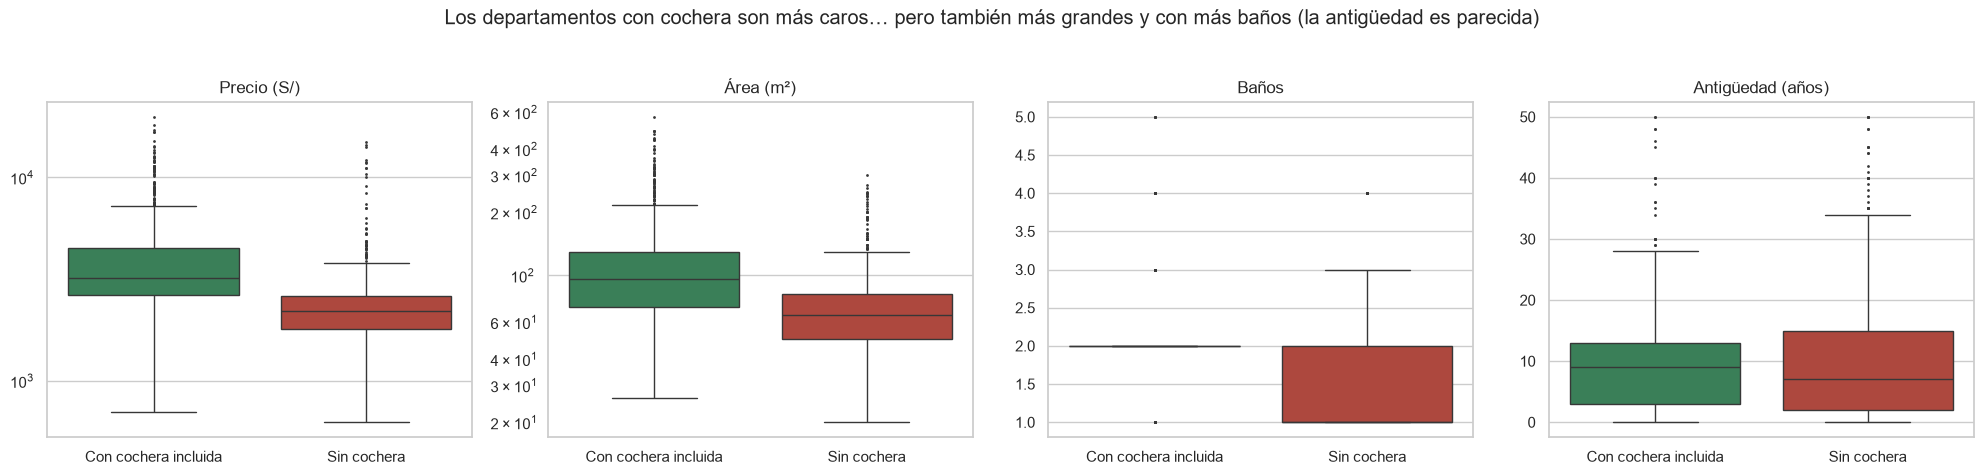
\includegraphics[width=\textwidth]{F0_eda_cochera_perfil.png}
\caption{Precio, área, baños y antigüedad de los avisos con y sin cochera incluida.}\label{fig:eda_perfil}
\origen{\texttt{notebook\_resumen.ipynb}, sección 2.2.}
\end{figure}

La cochera está repartida de forma muy desigual (figura~\ref{fig:coch_dist}): la incluye el 78\,\% de los avisos de Miraflores y el 68\,\% de los de San Isidro y Surco, frente al 20\,\% en San Miguel y el 15\,\% en Cercado. En los avisos que la cobran aparte, la mediana pedida es de \textbf{S/\,250 mensuales} (84 avisos en soles; rango intercuartil de S/\,200 a S/\,300). Es una referencia de mercado para la magnitud del efecto.

\begin{figure}[H]
\centering
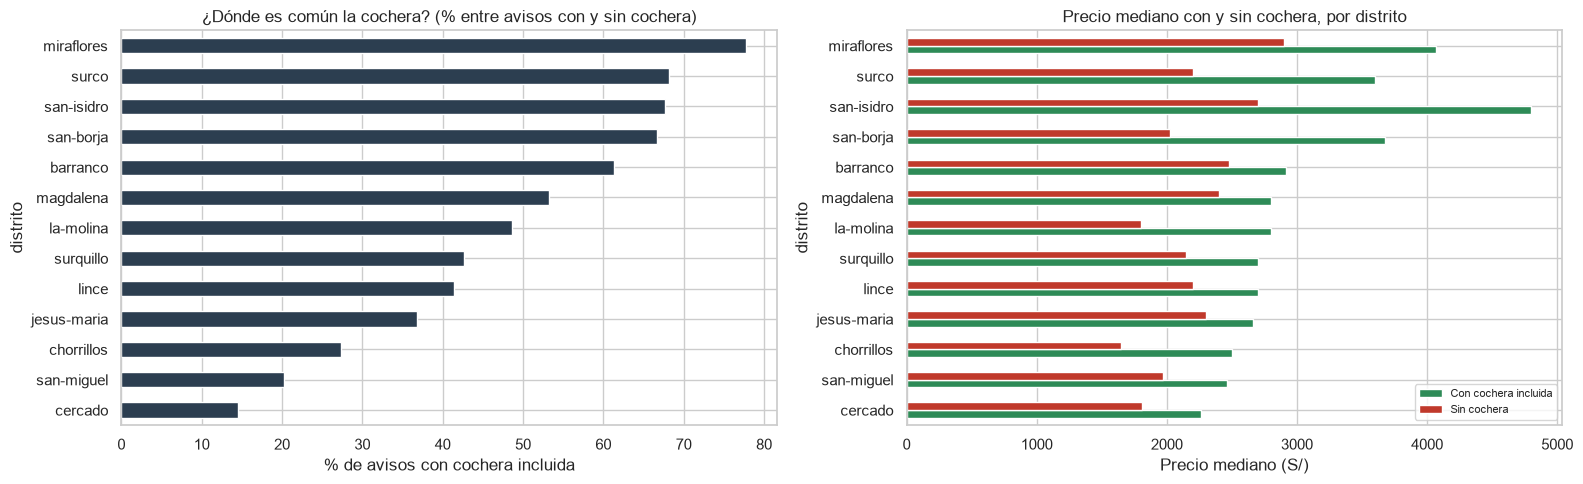
\includegraphics[width=\textwidth]{F0_eda_cochera_distrito.png}
\caption{Porcentaje de avisos con cochera incluida y alquiler mediano con y sin cochera, por distrito.}\label{fig:coch_dist}
\origen{\texttt{notebook\_resumen.ipynb}, sección 2.2.}
\end{figure}

\section{Soporte común y balance (R2)}\label{sec:res_soporte}

La propensión fuera de fold discrimina bien (AUC = 0.82; log-loss 0.52; Brier 0.17). Solo el 5\,\% de los avisos queda fuera de $[0.05,0.95]$, y el soporte común conserva 1\,949 avisos (1\,046 tratados y 903 controles). Antes de ponderar, las diferencias estandarizadas son grandes (0.92 en el área y 0.71 en los baños). Después, todas son menores que 0.05 en valor absoluto (figura~\ref{fig:soporte}): los grupos son comparables.

\begin{figure}[H]
\centering
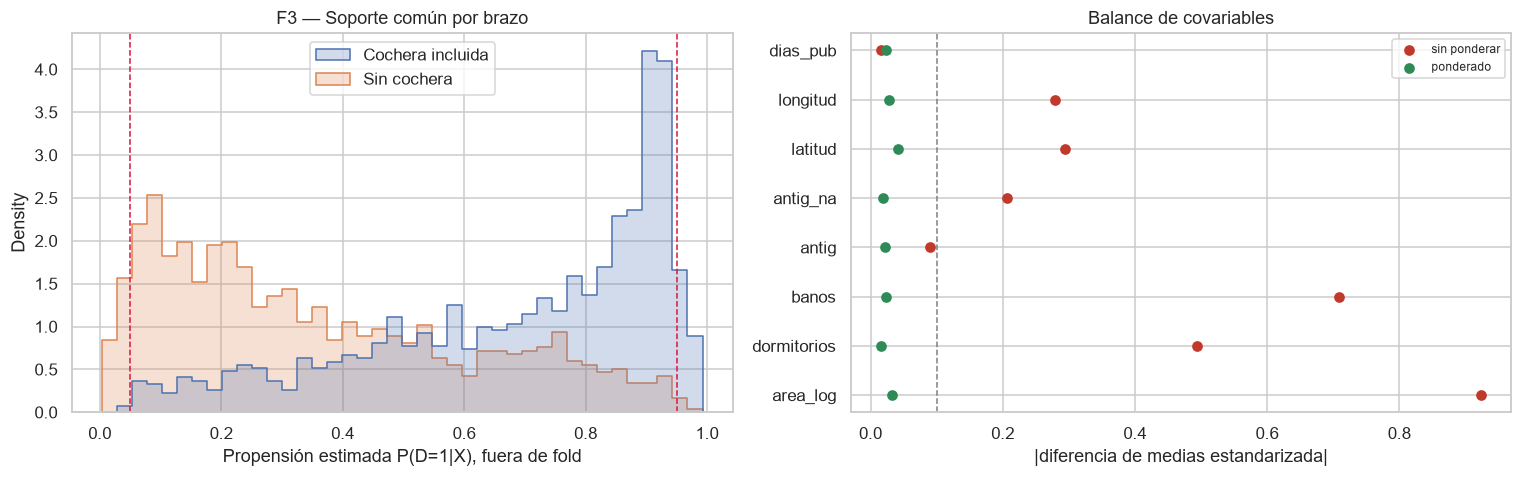
\includegraphics[width=0.95\textwidth]{F3_soporte_cochera.png}
\caption{Soporte común: propensión por grupo y balance antes y después de ponderar (R2).}\label{fig:soporte}
\origen{\texttt{notebook3b\_efecto\_cochera.ipynb}, sección 2 $\rightarrow$ \texttt{R2\_soporte.csv}, \texttt{R2\_balance.csv}.}
\end{figure}

\section{Efecto de la cochera incluida (R3)}\label{sec:res_efecto}

\begin{table}[H]
\centering\footnotesize
\caption{Efecto de tener cochera incluida sobre el precio de oferta (R3). EE agrupados por edificio}\label{tab:principal_c}
\resizebox{\textwidth}{!}{% Origen: notebook3b_efecto_cochera.ipynb -> resultados/tablas/R3c_principal.csv (generado por informe/tablas_manuscrito.py)
\begin{tabular}{lrrrcrcr}
\toprule
Estimador & N & $\theta$ & EE & IC 95\% ($\theta$) & \% efecto & IC 95\% (\%) & S/ al mes \\
\midrule
Diferencia sin ajustar (OLS) & 2,051 & 0.4883 & 0.0197 & [0.450, 0.527] & 63.0 & [56.8, 69.4] & 1,668 \\
Hedónico OLS & 2,051 & 0.0748 & 0.0133 & [0.049, 0.101] & 7.8 & [5.0, 10.6] & 206 \\
DML parcialmente lineal (PLR) & 2,051 & 0.0683 & 0.0119 & [0.045, 0.092] & 7.1 & [4.6, 9.6] & 187 \\
DML-IRM, muestra completa & 2,051 & 0.0425 & 0.0356 & [-0.027, 0.112] & 4.3 & [-2.7, 11.9] & 115 \\
DML-IRM, soporte común (principal) & 1,949 & 0.0724 & 0.0184 & [0.036, 0.108] & 7.5 & [3.7, 11.4] & 199 \\
\bottomrule
\end{tabular}}
\origen{\texttt{notebook3b\_efecto\_cochera.ipynb}, sección 3 $\rightarrow$ \texttt{R3c\_principal.csv}. Alquiler de referencia: S/\,2\,650.}
\end{table}

La diferencia bruta del 63\,\% se reduce, con el DML-IRM en el soporte común, a \textbf{7.5\,\% (IC 95\,\%: 3.7--11.4\,\%)}: unos \textbf{S/\,199 mensuales} (entre S/\,98 y S/\,303). El hedónico (7.8\,\%) y el PLR (7.1\,\%) coinciden. Sin recorte, el IRM es inestable (IC de $-2.7$ a 11.9\,\%), lo que confirma la necesidad del soporte común. Las 10 particiones dieron entre 6.8 y 9.4\,\%, y el modelo de precio explica el 82\,\% de la varianza fuera de fold. \textbf{H1 se confirma.}

\section{Grilla de especificaciones (R4)}\label{sec:res_grilla}

\begin{table}[H]
\centering\scriptsize
\caption{Efecto de la cochera bajo cada especificación (R4). DML-IRM, soporte común}\label{tab:especificaciones_c}
\resizebox{\textwidth}{!}{% Origen: notebook3b_efecto_cochera.ipynb -> resultados/tablas/R4c_especificaciones.csv (generado por informe/tablas_manuscrito.py)
\begin{tabular}{llp{3cm}rrrcr}
\toprule
Cód. & Especificación & Tipo & N & $\theta$ & EE & IC 95\% & \% efecto \\
\midrule
C1 & Principal & válida & 1,931 & 0.0732 & 0.0166 & [0.041, 0.106] & 7.6 \\
C2 & Sin área & omite confusor & 1,972 & 0.1081 & 0.0272 & [0.055, 0.161] & 11.4 \\
C3 & Sin ubicación (distrito, lat, lon) & omite confusor & 1,975 & 0.1961 & 0.0201 & [0.157, 0.236] & 21.7 \\
C4 & Sin baños ni dormitorios & omite confusor & 1,941 & 0.0868 & 0.0183 & [0.051, 0.123] & 9.1 \\
C5 & Sin antigüedad & omite confusor & 1,930 & 0.0775 & 0.0173 & [0.044, 0.111] & 8.1 \\
C6 & + precio/m$^2$ (descendiente de Y) & control inadmisible & 1,820 & -0.0046 & 0.0080 & [-0.020, 0.011] & -0.5 \\
C7 & Tratamiento estricto (incluida explícita) & medición & 547 & 0.0764 & 0.0342 & [0.009, 0.143] & 7.9 \\
C8 & Cochera con costo extra también como D=1 & medición & 2,113 & 0.0515 & 0.0156 & [0.021, 0.082] & 5.3 \\
C9 & + indicador de descripción cortada & medición & 1,926 & 0.0717 & 0.0181 & [0.036, 0.107] & 7.4 \\
P1 & Folds y EE por bloque de 1 km & partición & 1,953 & 0.0738 & 0.0204 & [0.034, 0.114] & 7.7 \\
\bottomrule
\end{tabular}}
\origen{\texttt{notebook3b\_efecto\_cochera.ipynb}, sección 4 $\rightarrow$ \texttt{R4c\_especificaciones.csv}.}
\end{table}

\begin{itemize}[itemsep=1pt]
\item \textbf{Confusores omitidos:} sin ubicación, el efecto casi se triplica (21.7\,\%), porque las cocheras abundan en las zonas caras. Sin área sube a 11.4\,\%.
\item \textbf{Control inadmisible:} el precio por m² lo anula ($-0.5$\,\%).
\item \textbf{Medición:} las alternativas se mueven en la dirección esperada. La definición estricta da 7.9\,\%, y contar las de costo extra como tratadas, 5.3\,\%.
\end{itemize}
El efecto se mueve mucho más con los controles que con el estimador (7.1--7.8\,\%). \textbf{H2 se confirma.}

\section{Robustez a confusores no observados (R5)}\label{sec:res_sens}

El valor de robustez es RV $=0.105$: un confusor que explique el 10.5\,\% de la variación residual de la cochera y del precio anularía el efecto. Para que el IC incluya el cero basta una fuerza de 0.054. Comparado con los observados (figura~\ref{fig:sensibilidad_c}), un confusor tan fuerte como la antigüedad llevaría el efecto a 0.4\,\%, y uno como la ubicación lo invertiría. La simulación muestra además que esta cota es optimista (sección~\ref{sec:res_sim}). El resultado es \textbf{frágil}. \textbf{H4 se confirma.}

\begin{figure}[H]
\centering
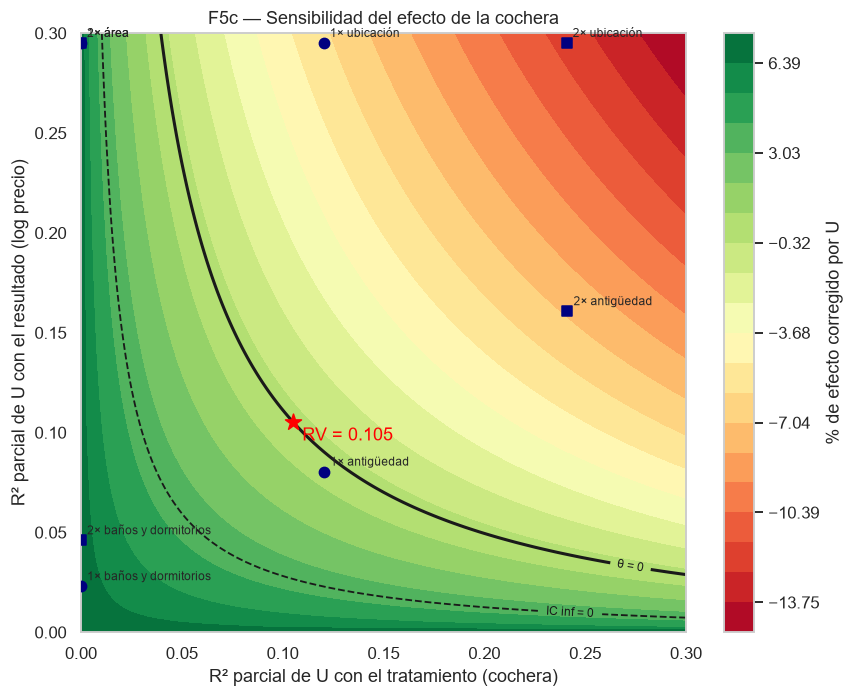
\includegraphics[width=0.6\textwidth]{F5c_sensibilidad_cochera.png}
\caption{Contorno de sensibilidad del efecto de la cochera con benchmarks observados (R5).}\label{fig:sensibilidad_c}
\origen{\texttt{notebook3b\_efecto\_cochera.ipynb}, sección 5 $\rightarrow$ \texttt{R5c\_sensibilidad.csv}.}
\end{figure}

\section{Heterogeneidad y dependencia espacial (R7)}\label{sec:res_het}

El efecto difiere por clase de distrito (figura~\ref{fig:gate_c}; Wald $\chi^2_2=18.3$, $p=0.0001$):
\begin{itemize}[itemsep=0pt]
\item \textbf{clase1} (Miraflores, San Isidro, Barranco, Lince): 1.5\,\%, con un IC que incluye el cero;
\item \textbf{clase2}: 10.3\,\%;
\item \textbf{clase3}: 17.8\,\%.
\end{itemize}
Por tamaño no hay diferencias ($p=0.35$). \textbf{H3 se confirma} por zona. Los residuos del precio tienen una autocorrelación espacial pequeña (I de Moran $=0.019$, $p=0.025$), y el IC agrupado por bloque de 1\,km también excluye el cero.

\begin{figure}[H]
\centering
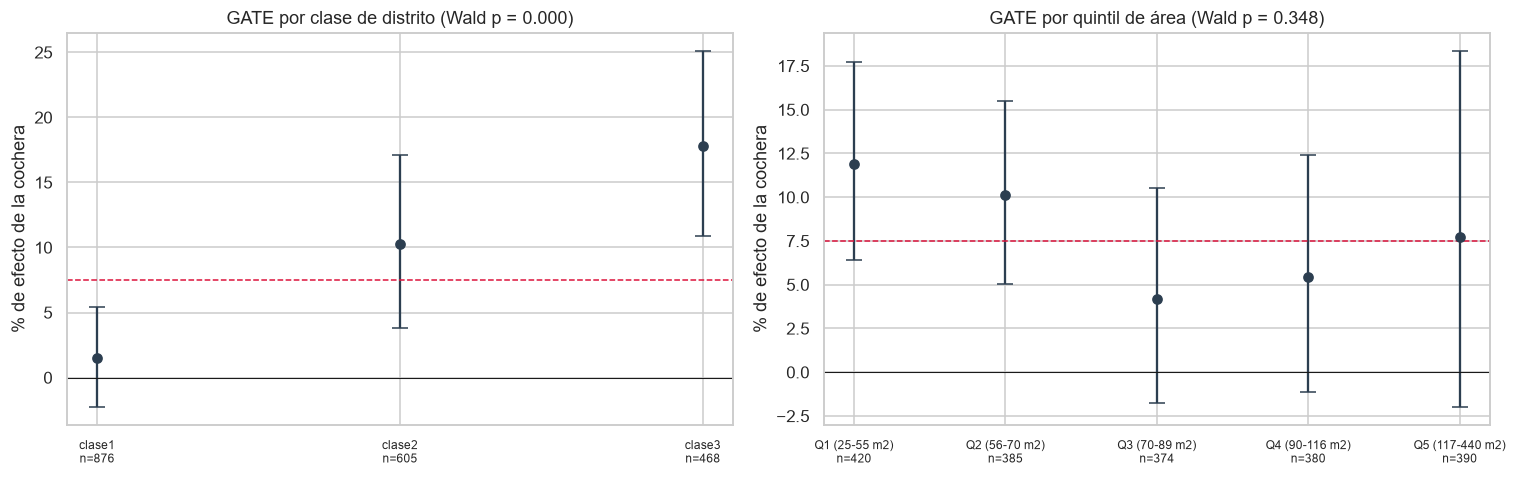
\includegraphics[width=\textwidth]{F7c_heterogeneidad_cochera.png}
\caption{Efecto de la cochera por clase de distrito y por quintil de área (R7).}\label{fig:gate_c}
\origen{\texttt{notebook3b\_efecto\_cochera.ipynb}, sección 6 $\rightarrow$ \texttt{R7c\_gate.csv}.}
\end{figure}

\section{Análisis secundario: un baño adicional}\label{sec:banos}

Con los mismos 2\,220 avisos (\texttt{notebook3\_estimacion\_causal}), la asociación bruta del 45.7\,\% se reduce a 7.4\,\% con el hedónico y a \textbf{3.8\,\% (IC 95\,\%: 1.7--6.0\,\%)} con el DML, unos S/\,100 mensuales:
\begin{itemize}[itemsep=0pt]
\item los \textit{learners} de árboles coinciden (3.8--4.4\,\%), mientras que Lasso, lineal, da 7.6\,\%;
\item sin área el efecto sube a 19.5\,\%, y con el precio por m² se anula;
\item agregar la cochera como control apenas lo cambia (3.5\,\%);
\item con todas las precisiones de geocodificación sube a 5.1\,\%: la ubicación imprecisa lo inflaba;
\item no hay heterogeneidad ($p>0.3$), y un confusor como la antigüedad lo dejaría en 0.7\,\% (RV = 0.079).
\end{itemize}

\section{Validación semisintética (R6)}\label{sec:res_sim}

\begin{table}[H]
\centering\small
\caption{Validación semisintética del estimador binario (100 réplicas por escenario; efecto verdadero 0.10)}\label{tab:sim_b}
\resizebox{0.85\textwidth}{!}{% Origen: notebook4_semisintetico.ipynb -> resultados/tablas/R6b_simulacion_binaria.csv (generado por informe/tablas_manuscrito.py)
\begin{tabular}{llrrrrr}
\toprule
Escenario & Estimador & $\theta$ verdadero & Sesgo & RMSE & Cobertura IC 95\% & Long. IC \\
\midrule
B1 & Hedónico OLS & 0.10 & 0.0002 & 0.0147 & 94 & 0.058 \\
B1 & DML PLR & 0.10 & -0.0040 & 0.0145 & 95 & 0.055 \\
B1 & DML-IRM (soporte común) & 0.10 & -0.0036 & 0.0198 & 96 & 0.081 \\
B2 & Hedónico OLS & 0.10 & 0.0412 & 0.0434 & 19 & 0.057 \\
B2 & DML PLR & 0.10 & 0.0392 & 0.0418 & 20 & 0.053 \\
B2 & DML-IRM (soporte común) & 0.10 & 0.0421 & 0.0462 & 45 & 0.078 \\
\bottomrule
\end{tabular}}
\origen{\texttt{notebook4\_semisintetico.ipynb} $\rightarrow$ \texttt{R6b\_simulacion\_binaria.csv}.}
\end{table}

\paragraph{Sin confusor omitido (B1).} Los tres estimadores recuperan el efecto: el sesgo es de 0.004 o menos y la cobertura del 94 al 96\,\%.

\paragraph{Con confusor moderado (B2).} Todos se sesgan ($\approx+0.04$) y la cobertura cae al 19--45\,\%. La cota de sensibilidad estimó un sesgo de 0.024 frente a uno real de 0.042, de modo que es \textbf{optimista} para el tratamiento binario.

\paragraph{Baños.} Para el estimador de baños, la simulación confirma tres cosas:
\begin{itemize}[itemsep=0pt]
\item sin confusor, el DML es insesgado (cobertura del 93\,\%), mientras que el hedónico lineal sobreestima el efecto (cobertura del 50\,\%);
\item con confusor, la cota sí es fiel (cobertura del 95--98\,\%);
\item la heterogeneidad real se detecta el 49\,\% de las veces.
\end{itemize}
